\section{Experimental Results}
\label{sec:experimental_results}
\subsection{Software Platform}
For our tests we are using \texttt{pandas},
a data manpilation librirary,
for reading data in structured formats such as
\texttt{.csv} and \texttt{.xlxs} files.
The AMIGOS dataset is avaible in \texttt{.mat} format.
As we would like to use Python for our work we used
the library \texttt{SciPi} to read this format in a Python friendly manner.
This library was also used for the signal processing portion of our project.
For ploting of figures we used \texttt{matplotlib.pyplot}.

\begin{figure*}[h]
    \centering
    \begin{subfigure}[t]{\columnwidth}
        \centering
        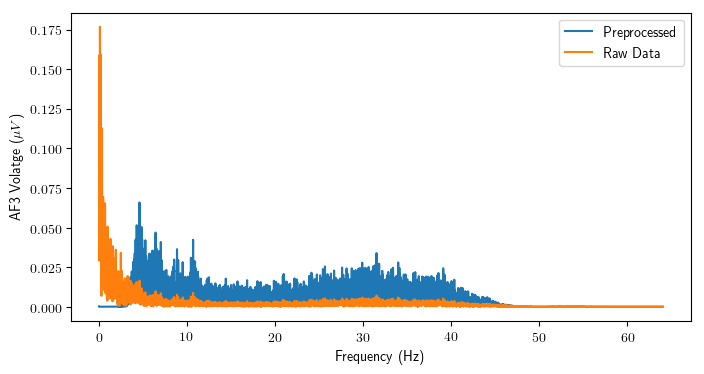
\includegraphics[width=\columnwidth]{tex/figures/filtering/AF3.png}
        \caption{AF3}
        \label{fig:filter:af3}
    \end{subfigure}
    \hfill
    \begin{subfigure}[t]{\columnwidth}
        \centering
        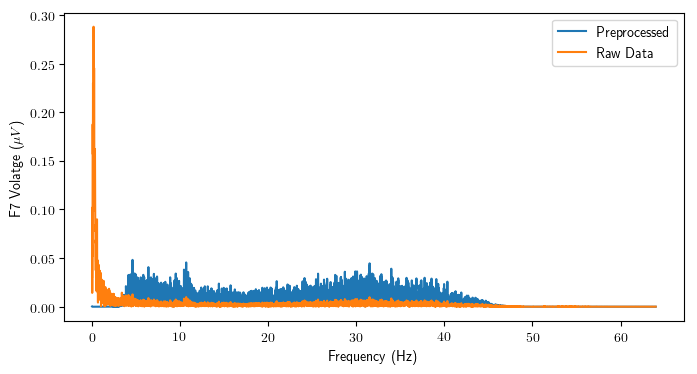
\includegraphics[width=\columnwidth]{tex/figures/filtering/F7.png}
        \caption{F7}
        \label{fig:filter:f7}
    \end{subfigure}
    \caption{Example filtering of EEG signal on sample 1 video 12}
    \label{fig:eeg}


    \begin{subfigure}[t]{\columnwidth}
        \centering
        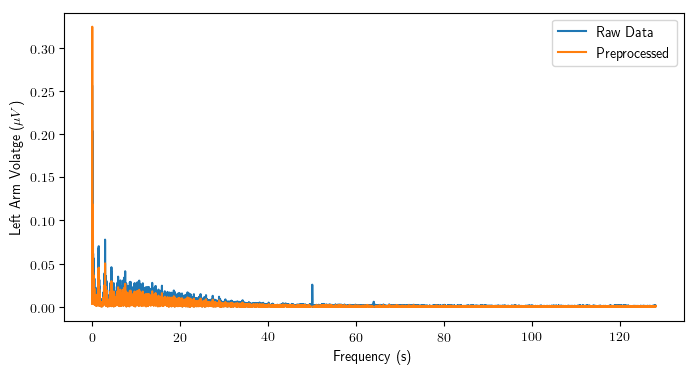
\includegraphics[width=\columnwidth]{tex/figures/filtering/ECG Left Arm.png}
        \caption{Left}
        \label{fig:filter:left}
    \end{subfigure}
    \hfill
    \begin{subfigure}[t]{\columnwidth}
        \centering
        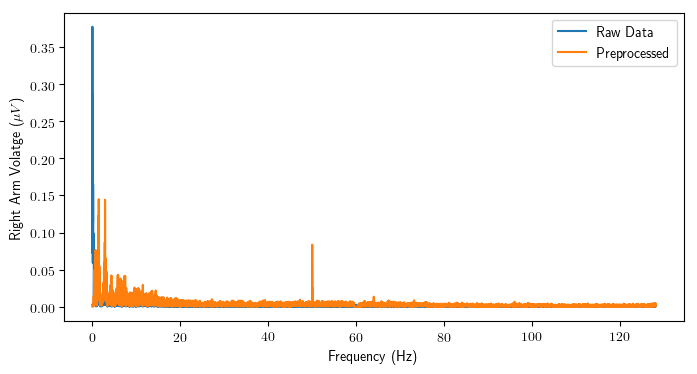
\includegraphics[width=\columnwidth]{tex/figures/filtering/ECG Right Arm.png}
        \caption{Right}
        \label{fig:filter:right}
    \end{subfigure}
    \caption{Example filtering of ECG signal on sample 1 video 12
             for the left and right arms}
    \label{fig:ecg}
\end{figure*}

\FloatBarrier
\subsection{Preprocessing}
We have applied 3 processing steps to our AMIGOS dataset;
signal filtering, [todo], and [todo].
In Figures \ref{fig:eeg} and \ref{fig:ecg}
we can see our filters applied to the EEG and ECG signals in the frequency domain.
For the EEG signal we followed the guideline set on the AMIGOS
website and applied a 4-45Hz bandpass filter \cite{AMIGOS:2018}.
We removed a significant amount of low frequency noise.
We can see that the preproccessed data results
in an slightly high amplitude than our original signal despite keeping the same shape.
Through experimental analysis we noticed that this was by a factor of 5.
For the ECG signal we applied a 0.05Hz highpass filter as noted in
\cite{SantamariaGranados:2019}
to remove baseline wander.
We also applied a bandstop filter with a 50Hz cutoff.
A small notch is visible in
Figures \ref{fig:filter:left} and \ref{fig:filter:right}.
The impact of the frequency filtering in the time domain can be seen in Figure
\label{fig:ecg:time}.

\clearpage

\begin{figure}[h]
    \centering
    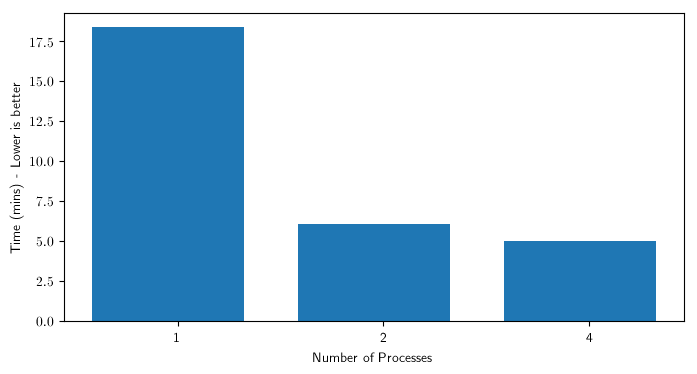
\includegraphics[width=\columnwidth]{tex/figures/multiprocess/multi_process_time.png}
    \caption{Time Taking to pre process data for different number of processes.}
    \label{fig:multip:time}
\end{figure}

\FloatBarrier
